   \documentclass{beamer}
\usepackage{color}
\usepackage{graphicx}
\usepackage{subcaption}
\usetheme{default}
\usepackage{cancel}
\usepackage[export]{adjustbox}[2011/08/13]
\setbeamercovered{transparent}
\usepackage[font={small}]{caption}
\usepackage{pdfcomment}
\newcommand{\pdfnote}[1]{\marginnote{\pdfcomment[icon=note]{#1}}}

\title{Nuclei Segmentation in Histopathology Images Using Deep Neural Networks}


\subtitle{Session: Histopathology Machine Learning}

\author{\textit{Peter Naylor}, Marick La\'e, Fabien Reyal and Thomas Walter}

\date{Friday April 21, 2017}

\subject{}


\begin{document}

\pdfnote{Hello everyone, my name is Peter Naylor and today I will }
\pdfnote{present our paper entitled "Nuclei Segmentation in }
\pdfnote{Histopathology Images Using Deep Neural Networks.}
\pdfnote{To briefly present the authors, Marick Laé and Fabien} \pdfnote{Reyal are two physicians and Thomas Walter is my supervisor}

\begin{frame}
  \titlepage
\end{frame}



\section{Introduction}


% me --> CBIO --> bioinformatics.
\pdfnote{I work in a bioinformatic group named CBIO in Paris and we mostly work on }
\pdfnote{cancer research related topics.} 
% bioinformatics --> omics data
\pdfnote{Bioinformaticians usually work on omics data, such as DNA copy number, mutations}
\pdfnote{or expression profiles.} 
\pdfnote{In particular in cancer research, the objective is often to}
\pdfnote{predict clinical variables such as prognosis or treatment response from omics data.}

\begin{frame}{Nuclei segmentation: why should you care?}
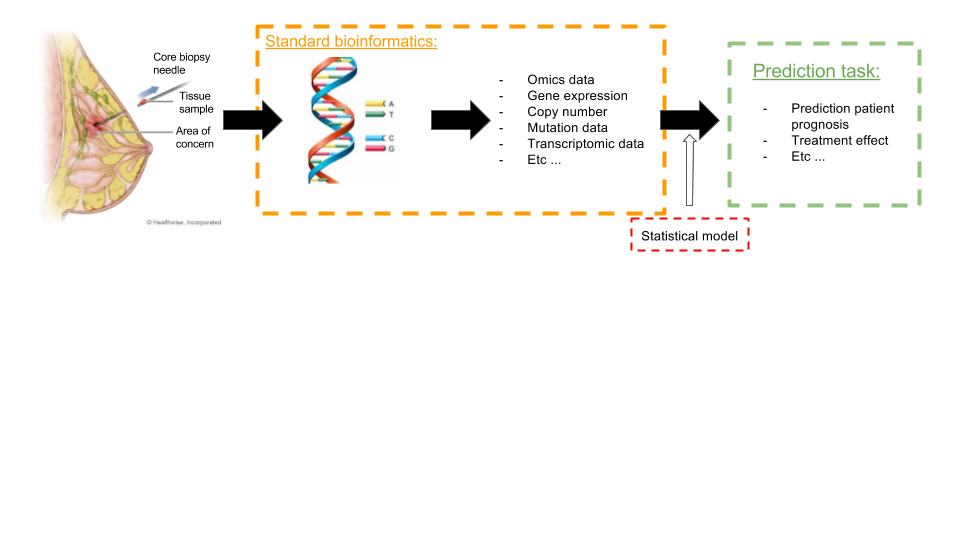
\includegraphics[width = 1.2\textwidth, center]{Standardbioinformatics.png}
\end{frame}
% our approach --> image data for prediction of clinical variables
\pdfnote{Our goal is to use histopathology images for such predictions.}

% Why images?
\pdfnote{Images contain valuable, complementary information with respect to other types of}
\pdfnote{genomic data.}
\pdfnote{
(1) images are informative about morphologies}
\pdfnote{
(2) images are informative about space}
\pdfnote{
(3) images are used already in clinical practice for diagnosis. }

% why segmentation of nuclei
%\pdfnote{ 1) We know that images contain a huge amount information.}
\pdfnote{ 1) How can we extract this relevant bioligical data?}
\pdfnote{ One way is to segment the nuclei, and from this detection we can extract}
\pdfnote{ 2) a) single cell data such as size of the nuclei, circularity just to name a few.}
\pdfnote{ 2) b) We can also account for more global features at the tissue level,}
\pdfnote{such as cell count, cell spatial distributions and global patterns.}
\pdfnote{ 3) Trying to create biologically relevant features. This is different just to maximizing a prediction accuracy.}


\begin{frame}{Nuclei segmentation: why should you care?}
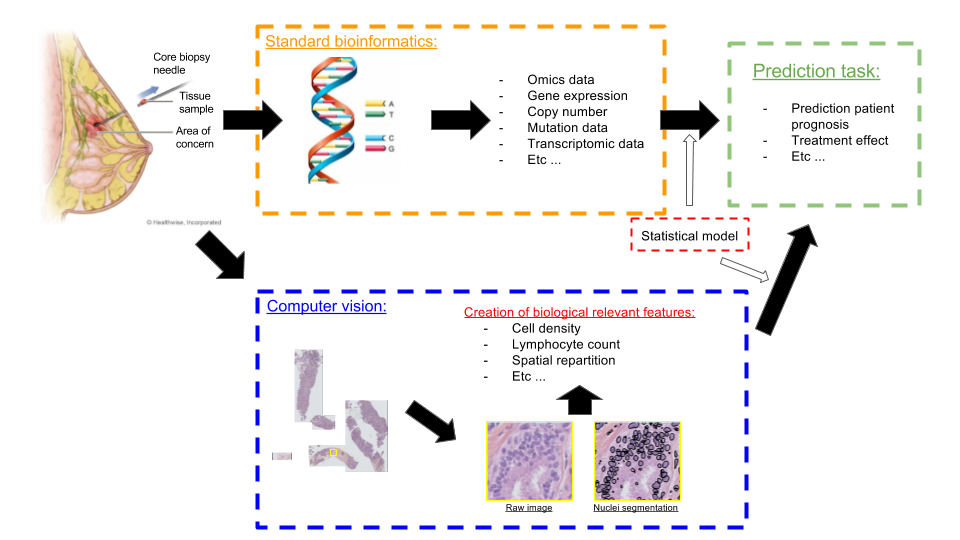
\includegraphics[width = 1.2\textwidth, center]{Whatido.png}
\end{frame}

\pdfnote{ -- Segmentation of nuclei is therefore a key step for such approaches}
\pdfnote{ -- but it remains a challenging problem. }
\pdfnote{ -- Due to the large variability in cell types, cell shapes, cell phase, }
\pdfnote{staining procedures and overall in real patients.}
\pdfnote{ -- As we can see in this mosaic that has been elaborated with only a}
\pdfnote{few patients, the variability in the image content can strongly vary}
\pdfnote{from one patient to another, but also within one patient. }

\pdfnote{ -- Many traditional methods, such as methods based on }
\pdfnote{Mathematical Morphology,
active contours and graph based methods have been proposed in the past.}
\pdfnote{ -- Such methods often work well on relatively homogeneous subsets of nuclei,}
\pdfnote{but have difficulties in coping with the large variability of nuclei illustrated here.}

\pdfnote{ -- We therefore decided to investigate the use of Deep Learning for nuclei segmentation.}

\pdfnote{ -- For this, the first thing we needed was a manually annotated data set that
covers the variability typically encountered in real data sets.}
\pdfnote{ -- The benefits of such a data set are thus two-fold: }
\pdfnote{(1) It can serve as a training set for supervised learning approaches.}
\pdfnote{(2) It can serve as a benchmark set for new methods.}

\pdfnote{ Conclusion: So we decided to produce a data set representative of}
\pdfnote{the high variability and make it publicly available.} 


\begin{frame}{Nuclei segmentation: challenging task}
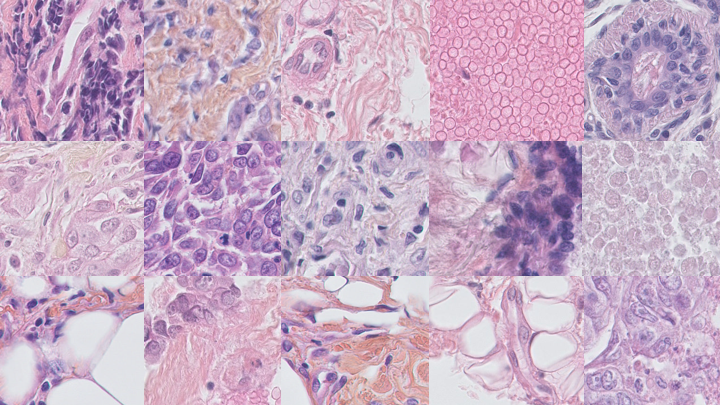
\includegraphics[width = 1.2\textwidth, center]{mosaique.png}
\end{frame}

\section{Data set elaboration for Nuclei segmentation}

\pdfnote{ -- You can download the dataset from my website.}
\pdfnote{ -- We tried to have a big variability between the different}
\pdfnote{samples and to exhaustively annotate them. }
\pdfnote{ -- To annotate each image we used an software named itk-snap.}
\pdfnote{ -- This software enabled us to annotate at a pixel level each one of the samples.}

\begin{frame}{Publicly available dataset for nuclei segmentation}

\begin{columns}
\vspace{-3cm}

\begin{column}{0.6\textwidth}
\begin{center}
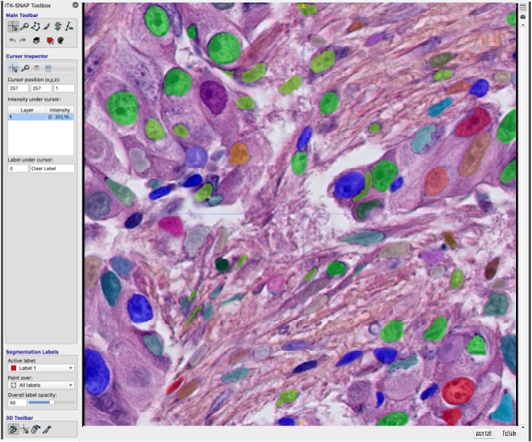
\includegraphics[scale = 0.5, center]{ITKSnap.png} \\
ITK-SNAP rendering, opacity: 50\% \\
\url{www.itksnap.org}
$\left[ \text{Yushkevich et Al 2006}\right]$
\end{center}
\end{column}

\begin{column}{0.5\textwidth}
\begin{small}
\begin{itemize}
\item High variability between samples
\item Benchmark dataset
\item Available at \url{PeterJackNaylor.github.io} 
\end{itemize}
\end{small}
\end{column}

\end{columns}

\end{frame}

\pdfnote{ -- Here are some statistics about available dataset.}

\begin{frame}{Cell Nuclei annotation}

\begin{itemize}
\item Manual annotation of Cell Nuclei.
\item 2754 annotated Cell Nuclei over 33 images.
\item 83 Cells on average (+/- 63 Cells). With a maximum of 297 cells.
\item 7 randomly choosen patients.
\item At least three 512 x 512 crops per patient.
\end{itemize}

\end{frame}

\pdfnote{ -- We are still updating this dataset and we have also added cell type.}
\pdfnote{ -- Now that we have a conveniant dataset we can start tunning}
\pdfnote{our statistical models.}

\begin{frame}{Cell Nuclei annotation, updated}
\begin{small}
\begin{itemize}
\item Manual annotation of Cell Nuclei.
\item \textcolor{red}{4022} \cancel{2754} annotated Cell Nuclei over \textcolor{red}{50} \cancel{33} images.
\item \textcolor{red}{80} \cancel{83} Cells on average (+/-  \textcolor{red}{58} \cancel{63} Cells). With a maximum of 297 cells.
\item  \textcolor{red}{11} \cancel{7} randomly choosen patients.
\item At least three 512 x 512 crops per patient.
\item Nuclei have been also classified in 8 classes: 
\end{itemize}
\end{small}

\begin{flushright}
\begin{footnotesize}
\begin{tabular}{|c|c|}
\hline 
Label & Counts \\ 
\hline 
Cancerous & 2206 \\ 
Lymphocyte/Plasmocyte & 896 \\ 
Fibroblast & 782 \\ 
Mitosis & 27 \\ 
Epithelial & 22 \\ 
%Necrose & 1 \\ 
Endothelial & 119 \\ 
Adiposite & 39 \\ 
\hline 
\end{tabular} 
\end{footnotesize}
\end{flushright}

\end{frame}

\section{Deep neural networks for segmentation}

\pdfnote{ -- Many people have manipulated deep neural network for segmentation.}
\pdfnote{ 1) Some have used them in a sliding window approach that we have}
\pdfnote{not tested for computation times.}
\pdfnote{ 2) We have mainly tried several architectures, one named pangnet (for the author)}
\pdfnote{which is a simple 3 layers, 8 feature maps per layer 
architecture.}
\pdfnote{ 3) We tried more elaborate architectures such as the FCN and deconvNet.}

\begin{frame}{Deep neural networks for segmentation}

\begin{columns}

\begin{column}{0.5\textwidth}
\begin{footnotesize}
Pixel wise classification. Many possible designs:
\begin{itemize}
\item Sliding window.
\item Series of convolution layers with no pooling. (PangNet) 
\item Learning upscalling (DeconvNet) 
\item Fusing down-scaling and up-scaling layers. (FCN) 
\end{itemize}
\end{footnotesize}

\begin{figure}
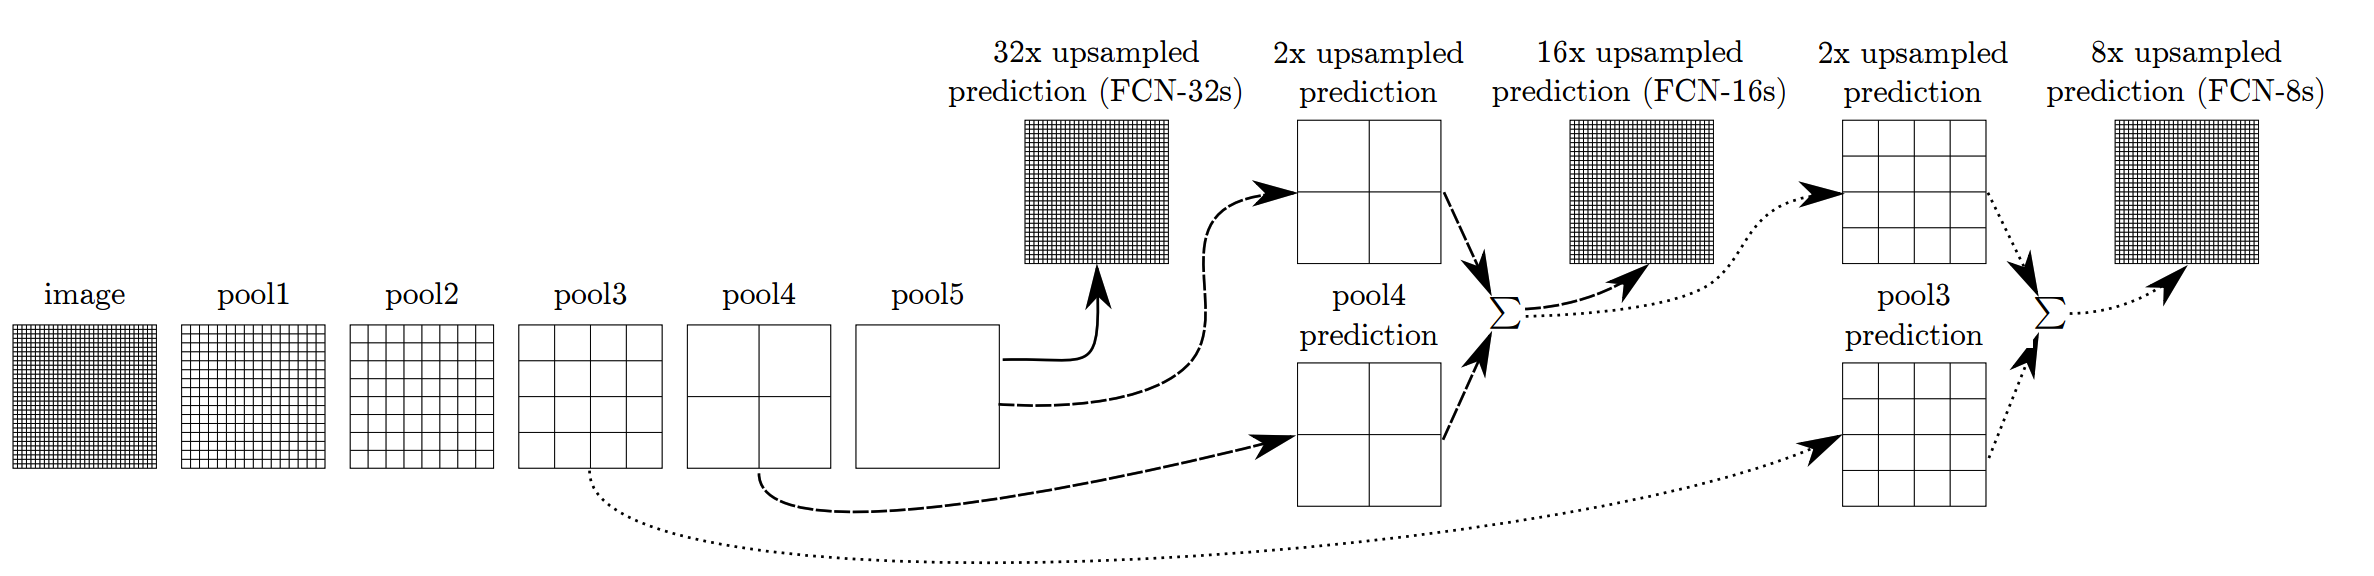
\includegraphics[width = 1.4\linewidth, left]{FCN.png}
\caption{FCN $\left[ \text{Long et Al 2014} \right]$}
\end{figure}

\end{column}

\begin{column}{0.5\textwidth}
\begin{figure}
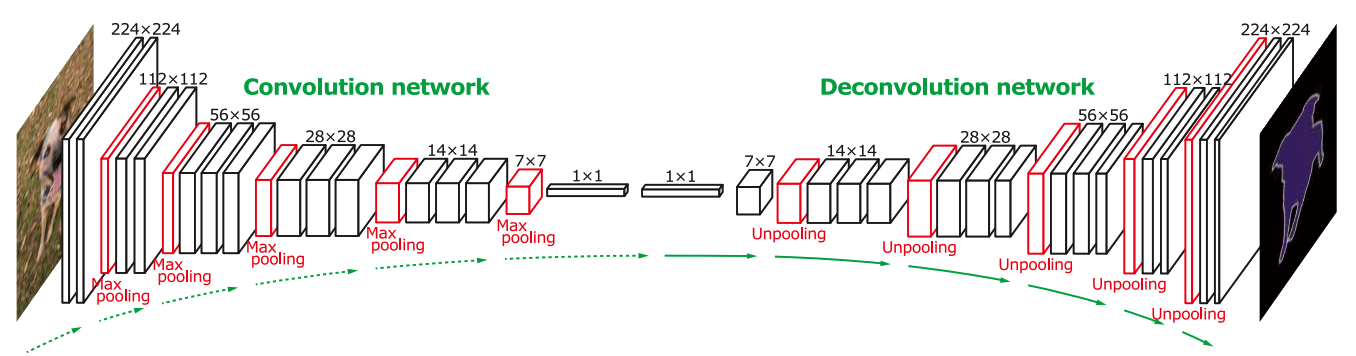
\includegraphics[width = 1.1\linewidth]{DeconvNet.png}
\caption{DeconvNet $\left[ \text{Noh et Al 2015} \right]$}
\end{figure}


\begin{figure}
\hspace{2cm }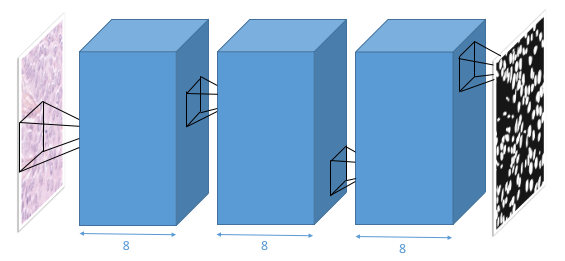
\includegraphics[width = 0.5\linewidth]{PangNet.png}
\caption{PangNet  $\left[ \text{Pang et Al 2010}\right]$}
\end{figure}

\end{column}
\end{columns}




\end{frame}


\section{Post-processing the probability map}

\pdfnote{ -- I want to first bring your attention to the probability map}
\pdfnote{this a typical output for a well trained networks.}
\pdfnote{ -- We can notice several things:}
\pdfnote{ 1) First, DNN seem to be very good at distinguishing between }
\pdfnote{foreground and background.}
\pdfnote{ 2) Secondly, sadly for us, they seem pretty bad at seperating }
\pdfnote{cluttered cells or touching cells.}
\pdfnote{ -- We therefore add post-processing step in order to help the }
\pdfnote{network seperate cells.}

\begin{frame}{Post-processing method for the probability map}

\only<1>{
\begin{figure}
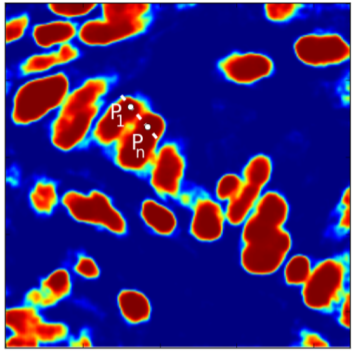
\includegraphics[width = 0.7\linewidth, center]{ProbabilityMap.png} 
\caption{Typical probability map of a trained neural network \\ 
\hspace{3cm} (in particular: FCN)
 }
\end{figure}
}


\only<2>{We notice that, the posterior probability at the nucleus border is systematically lower than in the putative center of the nucleus.
\\
%%Candidates for the center of the nucleus: local maximum a posteriori. \\
Let $\mathcal{P}$ be the all possible probability pathways from two candidates $P_1$ and $P_N$ (two maximum a posteriori). We split if: 
$$\min_{\mathcal{P}}C(\mathcal{P}) = \min_{\mathcal{P}} \{\max_{i=2
  \ldots N}{p_1-p_i}\} > \lambda$$}

\only<2>{\begin{figure}
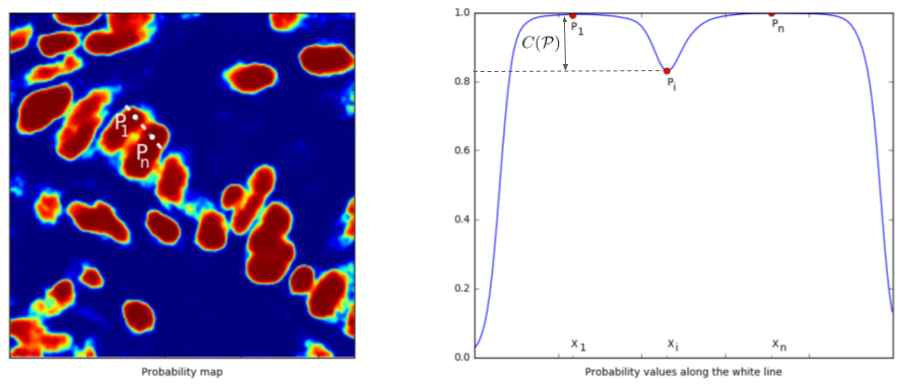
\includegraphics[width = \linewidth]{WS.png} 
\caption{Values along one arbitrary path between two candidates.}
\end{figure}
}

\end{frame}




\section{Results}
\pdfnote{ -- Several remarks: On the probability output}
\pdfnote{ 1) PangNet is too simple, it learns to simple decision, such as pixel color values}
\pdfnote{ , in particular dark purple.}
\pdfnote{ 2) Sacrificing resolution seems to help the networks better understand the concept of cell}
\pdfnote{ -- It is evident that this post-processing step is highly depended }
\pdfnote{on the probability output.} 
\pdfnote{ -- A very bumpy probability map will lead to a very poor final segmentation.}
\pdfnote{ -- If the probability map is well suited. The parameter lambda can be adjusted,}
\pdfnote{if too low: over segmentation, if too high: we won't be seperating cells.}


\begin{frame}{Visual Results}

\begin{columns}
\begin{column}{0.3\textwidth}
\begin{figure}
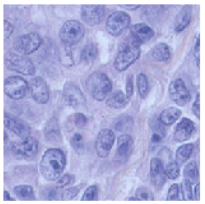
\includegraphics[width = 0.8\linewidth]{RAW} 
\caption{Input}
\end{figure}

\begin{figure}
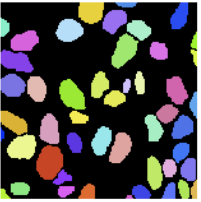
\includegraphics[width = 0.8\linewidth]{LBL} 
\caption{Ground Truth}
\end{figure}

\end{column}
\begin{column}{0.7\textwidth}
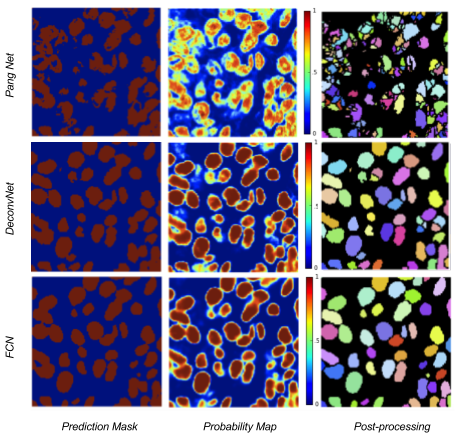
\includegraphics[width=1.1\textwidth]{Test}

\end{column}
\end{columns}
\end{frame}
\begin{frame}{Results summary}
\begin{small}
\begin{tabular}{r|c|c|c|c|c|}
     &        FCN &     DeconvNet  & PangNet & Ensemble \\
\hline
Accuracy           &        0.942 (\textcolor{red}{0.955}) &     0.955 (\textcolor{red}{0.952}) &       0.925 & 0.944  (\textcolor{red}{0.953})  \\
Performance      &        0.873 (\textcolor{red}{0.889}) &     0.877 (\textcolor{red}{0.873}) &       0.806 & 0.922 (\textcolor{red}{0.926}) \\
IU                      &        0.787 (\textcolor{red}{0.823}) &     0.820 (\textcolor{red}{0.814}) &       0.720 & 0.804 (\textcolor{red}{0.825}) \\
Recall                &        0.781 (\textcolor{red}{0.799})  &     0.774 (\textcolor{red}{0.767}) &        0.655 & 0.900 (\textcolor{red}{0.896}) \\
Precision            &        0.784 (\textcolor{red}{0.861}) &     0.867 (\textcolor{red}{0.864}) &        0.784 & 0.741 (\textcolor{red}{0.777})  \\
F1                     &        0.776 (\textcolor{red}{0.828}) &     0.818 (\textcolor{red}{0.811}) &       0.675 & 0.802 (\textcolor{red}{0.825}) \\
\end{tabular} 
\\
\textit{In red are the results with the additionnal data.}
\end{small}

\begin{columns}

\begin{column}{0.5\textwidth}
\begin{figure}
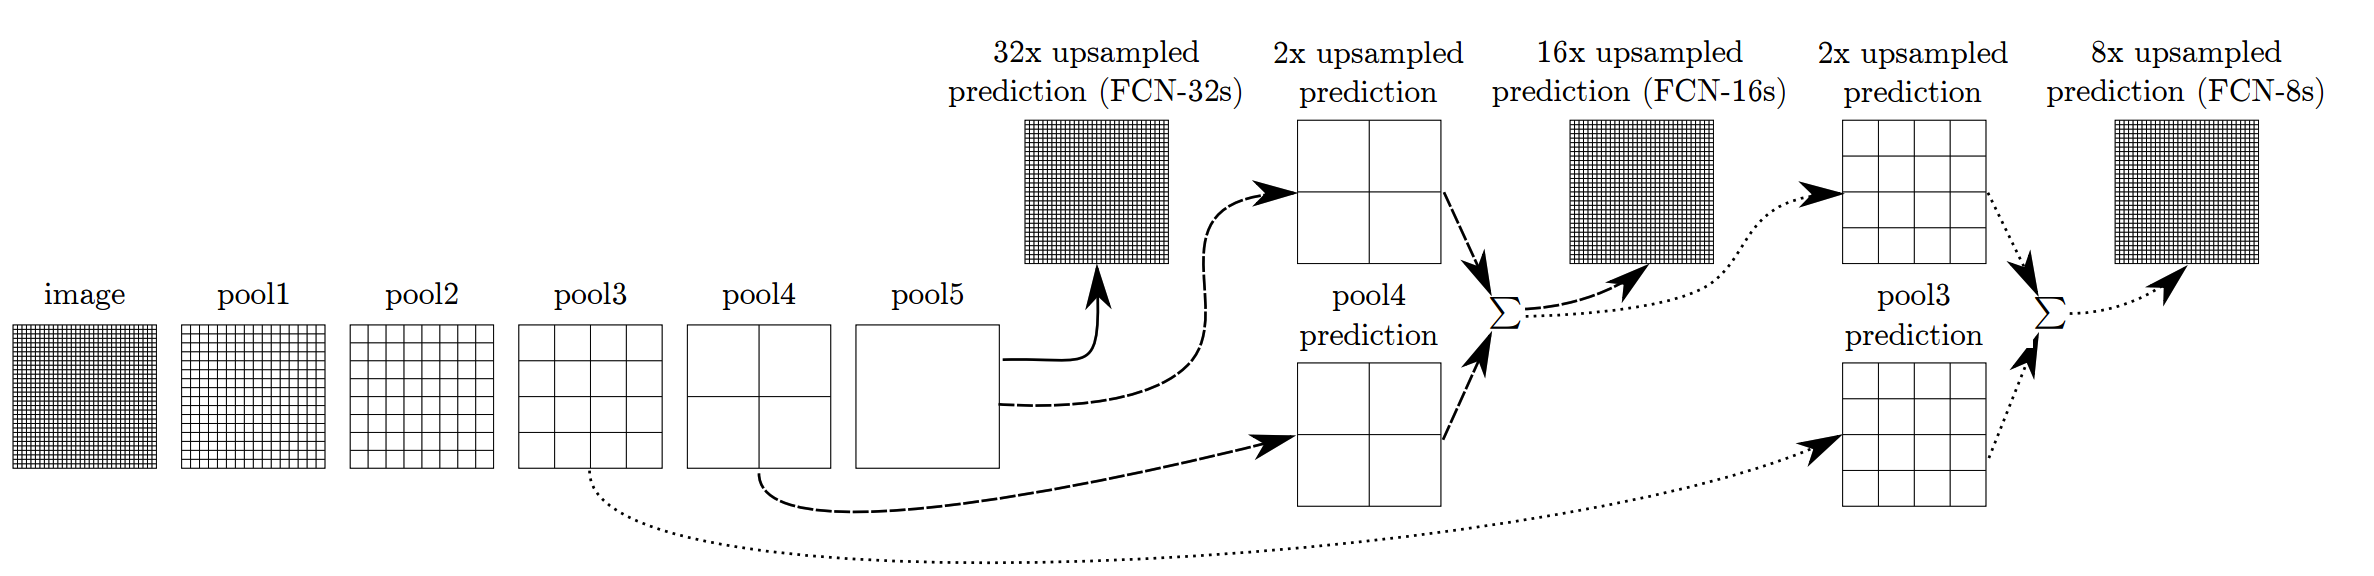
\includegraphics[width = 1.12\linewidth, left]{FCN.png}
\caption{FCN}
\end{figure}
\end{column}

\begin{column}{0.3\textwidth}
\begin{figure}
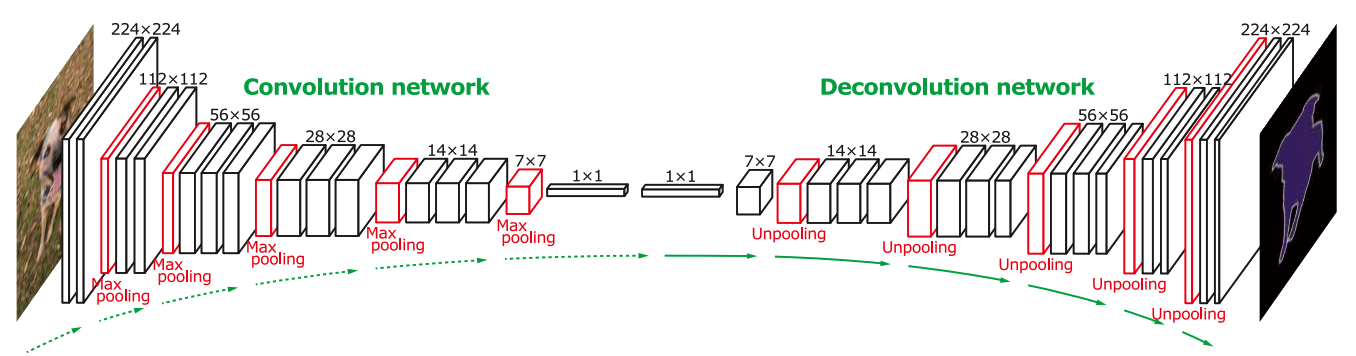
\includegraphics[width = 1.1\linewidth]{DeconvNet.png}
\caption{DeconvNet}
\end{figure}
\end{column}

\begin{column}{0.3\textwidth}
\begin{figure}
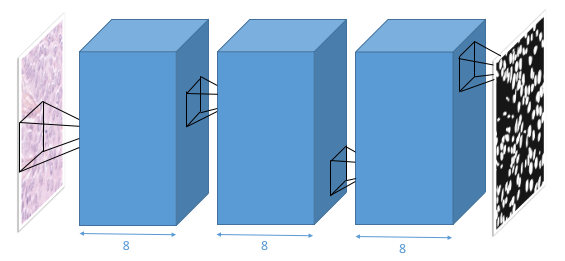
\includegraphics[width = 0.7\linewidth]{PangNet.png}
\caption{PangNet}
\end{figure}
\end{column}

\end{columns}

\end{frame}

\begin{frame}{Conclusion}
3 fold contributions for this paper:
\begin{itemize}
\item Publicly available dataset.
\item Benchmark results with recent deep neural network architectures.
\item Post-processing scheme for dealing with touching cells.
\end{itemize}

\end{frame}

\pdfnote{No notes for the perspectiv yet}
\pdfnote{ -- Interest in nuclei segmentation: allows for biological driven analysis/understanding of patient treatment.}


\begin{frame}{Perspectives}

\begin{figure}
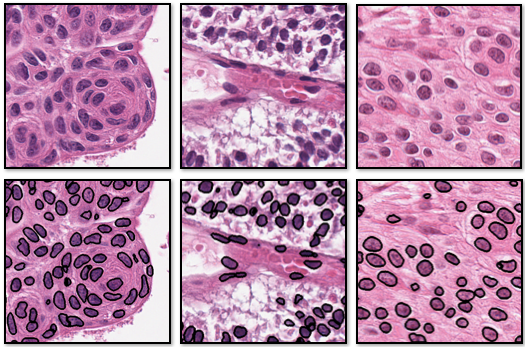
\includegraphics[width = 0.8\linewidth]{bladdercancer.png} 
\caption{Bladder cancer}
\end{figure}

\end{frame}

\end{document}

